\documentclass[tikz,border=10pt]{standalone}
\usepackage{tikz}
\begin{document}
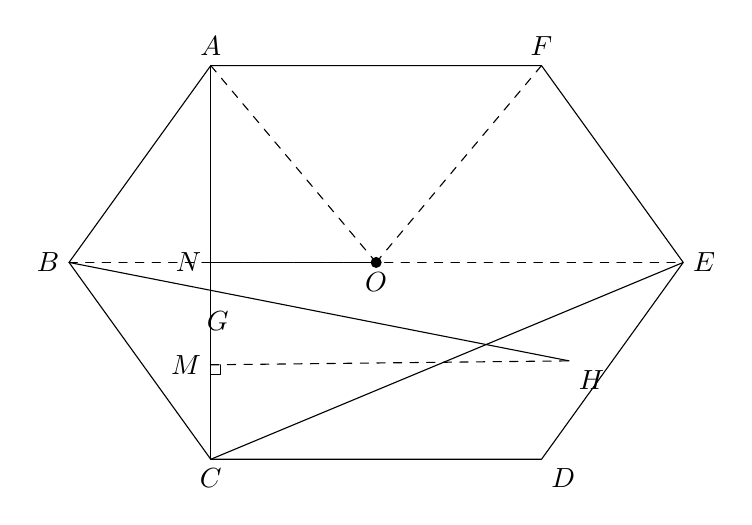
\begin{tikzpicture}[line cap=round,line join=round,scale=1]

% Coordinates
\coordinate (A) at (0,4);
\coordinate (F) at (4.2,4);
\coordinate (E) at (6,1.5);
\coordinate (D) at (4.2,-1);
\coordinate (C) at (0,-1);
\coordinate (B) at (-1.8,1.5);

\coordinate (O) at (2.1,1.5);
\coordinate (N) at (0,1.5);
\coordinate (M) at (0,0.2);
\coordinate (G) at (0.35,0.75);
\coordinate (H) at (4.55,0.25);

% Outer hexagon
\draw (A)--(F)--(E)--(D)--(C)--(B)--cycle;

% Interior solid segments
\draw (A)--(C);
\draw (B)--(H);
\draw (C)--(E);

% Dashed segments
\draw[dashed] (B)--(E);
\draw[dashed] (N)--(O);
\draw[dashed] (M)--(H);
\draw[dashed] (A)--(O);
\draw[dashed] (F)--(O);

% Point O
\fill (O) circle (2pt);

% Right-angle mark at M
\draw (0,0.2) ++(0.12,0) -- ++(0,-0.12) -- ++(-0.12,0);

% Labels
\node[above] at (A) {$A$};
\node[above] at (F) {$F$};
\node[right] at (E) {$E$};
\node[below right] at (D) {$D$};
\node[below] at (C) {$C$};
\node[left] at (B) {$B$};

\node[below] at (O) {$O$};
\node[left] at (N) {$N$};
\node[left] at (M) {$M$};
\node[left] at (G) {$G$};
\node[below right] at (H) {$H$};

\end{tikzpicture}
\end{document}
